\documentclass[11pt]{article}
\usepackage[utf8]{inputenc}
\usepackage[dvips]{graphicx}
\usepackage{fancybox}
\usepackage{verbatim}
\usepackage{multirow,array}
\usepackage{latexsym}
\usepackage{alltt}
\usepackage{hyperref}
\usepackage{textcomp}
\usepackage{color}
\usepackage{amsmath}
\usepackage{amsfonts}
\usepackage{tikz}
\usepackage{float}
\usepackage[hmargin=3cm,vmargin=5.0cm]{geometry}
%\topmargin=0cm
\topmargin=-2cm
\addtolength{\textheight}{6.5cm}
\addtolength{\textwidth}{2.0cm}
%\setlength{\leftmargin}{-5cm}
\setlength{\oddsidemargin}{0.0cm}
\setlength{\evensidemargin}{0.0cm}

\newcommand{\scale}[0] {2}
\newcommand{\scle}[0] {1}


\begin{document}

\section*{Student Information } 
%Write your full name and id number between the colon and newline
%Put one empty space character after colon and before newline
Full Name : Batuhan Karaca \\
Id Number : 2310191 \\

% Write your answers below the section tags

\section*{Answer 1}
\subsection*{a)}

    

\begin{figure}[H]
    
    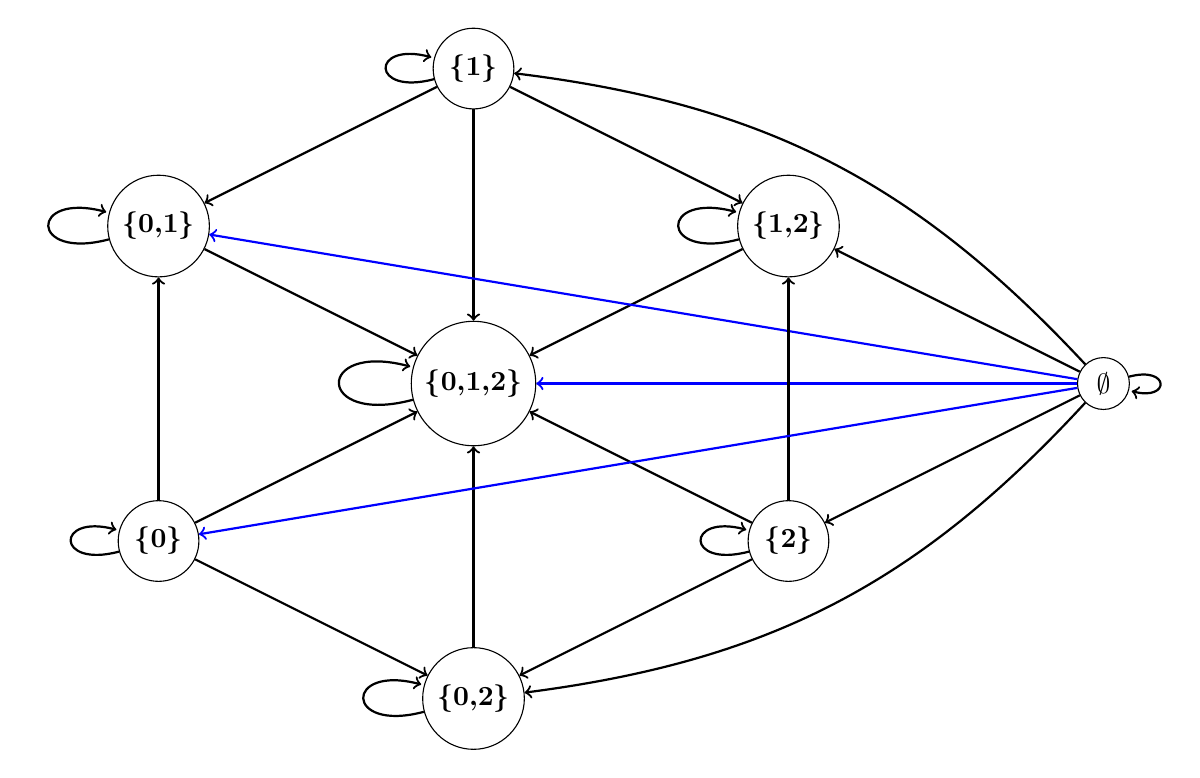
\begin{tikzpicture}
        \node[shape=circle,draw=black] (a) at (0, 0)     { \textbf{\{0,1,2\}} };
        \node[shape=circle,draw=black] (b) at (-\scale*2, \scale)     {\textbf{\{0,1\}}};
        \node[shape=circle,draw=black] (c) at (\scale*2, \scale)     {\textbf{\{1,2\}}};
        \node[shape=circle,draw=black] (d) at (0, -\scale*2)     {\textbf{\{0,2\}}};
        \node[shape=circle,draw=black] (e) at (-\scale*2, -\scale)     {\textbf{\{0\}}};
        \node[shape=circle,draw=black] (f) at (0,\scale*2)     {\textbf{\{1\}}};
        \node[shape=circle,draw=black] (g) at (\scale*2, -\scale)     {\textbf{\{2\}}};
        \node[shape=circle,draw=black] (h) at (\scale*4, 0)     {\textbf{$\emptyset$}};
        
        %subsets of a
        \path[->, thick] (a) edge [loop left] (a);
        \path[->, thick] (b) edge (a);
        \path[->, thick] (c) edge (a);
        \path[->, thick] (d) edge (a);
        \path[->, thick] (e) edge (a);
        \path[->, thick] (f) edge (a);
        \path[->, thick] (g) edge (a);
        \path[->, thick, blue] (h) edge (a);  
       
        %subsets of b
        \path[->, thick] (b) edge [loop left] (b);
        \path[->, thick] (e) edge (b);
        \path[->, thick] (f) edge (b);
        \path[->, thick, blue] (h) edge (b);

        %subsets of c
        \path[->, thick] (c) edge [loop left] (c);
        \path[->, thick] (f) edge (c);
        \path[->, thick] (g) edge (c);
        \path[->, thick] (h) edge (c);

        %subsets of d
        \path[->, thick] (d) edge [loop left] (d);
        \path[->, thick] (e) edge (d);
        \path[->, thick] (g) edge (d);
        \path[->, thick] (h) edge [bend left=20] (d);

        %subsets of e
        \path[->, thick] (e) edge [loop left] (e);
        \path[->, thick, blue] (h) edge (e);

        %subsets of f
        \path[->, thick] (f) edge [loop left] (f);
        \path[->, thick] (h) edge [bend right=20] (f);

        %subsets of g
        \path[->, thick] (g) edge [loop left] (g);
        \path[->, thick] (h) edge (g);
        
        %subsets of h
        \path[->, thick] (h) edge [loop right] (h);
        

	\end{tikzpicture}

\end{figure}
\subsection*{b)}
In order that $(S,R)$ is poset, $R$ needs to be a partial ordering on $S$. Then, $R$ needs to be
\begin{enumerate}
    \item reflexive
    \item antisymmetric
    \item transitive
\end{enumerate}
\textbf{1)reflexivity}
\\ \\
For all $s$ in $S$, $s$ is a set, since the set $S$ is the power set of another set.
Every set is a subset of itself. Then $s$ is a subset of itself. Then $(s,s) \in R$.
We proved for all $s \in S$, $(s,s) \in R$. Then $R$ is reflexive.
\\ \\
\textbf{2)antisymmetry}
\\ \\
For any sets $s_1$ and $s_2$, if $s_1 \subseteq s_2$ and $s_2 \subseteq s_1$, then $s_1 = s_2$.
Then for any sets $s_1$ and $s_2$ in $S$, if $(s_1,s_2) \in R$, $s_1 \subseteq s_2$ and if 
$(s_2,s_1) \in R$, $s_2 \subseteq s_1$. Then $s_1=s_2$, hence $R$ is antisymmetric.
\\ \\
\textbf{3)transitivity}
\\ \\
For any sets $s_1$,$s_2$ and $s_3$, if $s_1 \subseteq s_2$ and $s_2 \subseteq s_3$, then $s_1 
\subseteq s_3$. Then for any sets $s_1$,$s_2$ and $s_3$ in $S$, if $(s_1,s_2) \in R$, $s_1 \subseteq s_2$ 
and if $(s_2,s_3) \in R$, $s_2 \subseteq s_3$. Then $s_1 \subseteq s_3$, hence $(s_1,s_3) \in R$. 
Hence $R$ is transitive.
\\ \\
$R$ is a partial ordering on $S$, hence $(S,R)$ is a poset.
\\ \\
\subsection*{c)}
From the textbook(Eighth Edition) page 651
\\ \\
\begin{tabular}{l}
    \textit{The elements $a$ and $b$ of a poset $(S,R)$ are called comparable if either $aRb$ or $bRa$.}   
\end{tabular}
\\ \\
\begin{tabular}{l}
    \textit{If $(S,R)$ is a poset and every two elements of $S$ are comparable, $(S,R)$ is a total order.} 
\end{tabular}
\\ \\
Assume $a=\{1,2\} \in S$ and $b=\{0,1\} \in S$. Then neither $a \subseteq b$ nor $b \subseteq a$. Then 
$a$ and $b$ are incomparable. Since there is at least two elements that are not comparable within, in $S$;
by contradiction, $(S,R)$ is not a total order. 

\subsection*{d)}
\begin{figure}[H]
    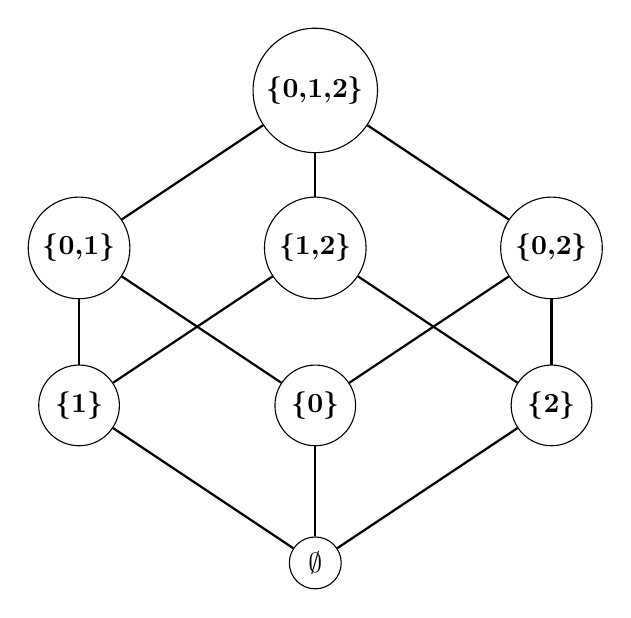
\begin{tikzpicture}
        \node[shape=circle,draw=black] (a) at (0, \scle*3)     { \textbf{\{0,1,2\}} };
        \node[shape=circle,draw=black] (b) at (-\scle*3, \scle)     {\textbf{\{0,1\}}};
        \node[shape=circle,draw=black] (c) at (0, \scle)     {\textbf{\{1,2\}}};
        \node[shape=circle,draw=black] (d) at (\scle*3, \scle)     {\textbf{\{0,2\}}};
        \node[shape=circle,draw=black] (e) at (0, -\scle)     {\textbf{\{0\}}};
        \node[shape=circle,draw=black] (f) at (-\scle*3,-\scle)     {\textbf{\{1\}}};
        \node[shape=circle,draw=black] (g) at (\scle*3, -\scle)     {\textbf{\{2\}}};
        \node[shape=circle,draw=black] (h) at (0, -\scle*3)     {\textbf{$\emptyset$}};
        
        %subsets of a
        \path[-, thick] (a) edge (b);
        \path[-, thick] (a) edge (c);
        \path[-, thick] (a) edge (d);

        \path[-, thick] (b) edge (e);
        \path[-, thick] (b) edge (f);

        \path[-, thick] (d) edge (e);
        \path[-, thick] (d) edge (g);

        \path[-, thick] (c) edge (f);
        \path[-, thick] (c) edge (g);

        \path[-, thick] (h) edge (e);
        \path[-, thick] (h) edge (f);
        \path[-, thick] (h) edge (g);
	\end{tikzpicture}
\end{figure}

\subsection*{e)}
From the textbook(Eighth Edition) page 657
\\ \\
\begin{tabular}{l}
    \textit{If $u$ is an element of $S$ such that $aRu$ for all elements $a \in A$, then $u$ is called an upper bound of $A$.} \\
    \textit{If $l$ is an element of $S$ such that $lRa$ for all elements $a\in A$, then $l$ is called a lower bound of $A$.} (1)
\end{tabular}
\\ \\
\begin{tabular}{l}
    \textit{The element $x$ is called the least upper bound of the subset $A$ if x is an upper bound that is less than} \\
    \textit{every other upper bound of $A$. Similarly, the element $y$ is called the greatest lower bound of $A$ if $y$} \\
    \textit{is a lower bound of $A$ and $zRy$ whenever $z$ is a lower bound of $A$.} (2)
\end{tabular}
\\ \\
From the textbook(Eighth Edition) page 658
\\ \\
\begin{tabular}{l}
    \textit{A partially ordered set in which every pair of elements has both a least upper bound and a greatest} \\
    \textit{lower bound is called a lattice.} (3)
\end{tabular}
\\ \\
$(S,R)$ is a poset from part \textbf{(b)}. Assume subsets $s_1$ and $s_2$, $s_{max}$, $s_{min}$ 
of $S$ given, such that $s_1 \subseteq s_{max}$ and $s_2 \subseteq s_{max}$ and $s_{min} \subseteq s_1$ 
and $s_{min} \subseteq s_2$. Then by the definition(s) $(1)$, $s_{min}$ is a lower bound and $s_{max}$ 
is an upper bound for the set $\{s_1, s_2\}$. If $s_{max}$ is the least of all upper bounds, 
then $s_{max}=s_1 \cup s_2$, similiarly if $s_{min}$ is the greatest of all lower bounds, then 
$s_{min}=s_1 \cap s_2$.For all $s_1, s_2$ in $S$, we can find such $s_{max},\ s_{min}$. Then every 
pair $(s_1,s_2) \in R$ has both a least upper bound and a greatest lower bound. Hence $(S,R)$ 
constitutes a lattice.
\section*{Answer 2}
\subsection*{a)}
\begin{figure}[H]
    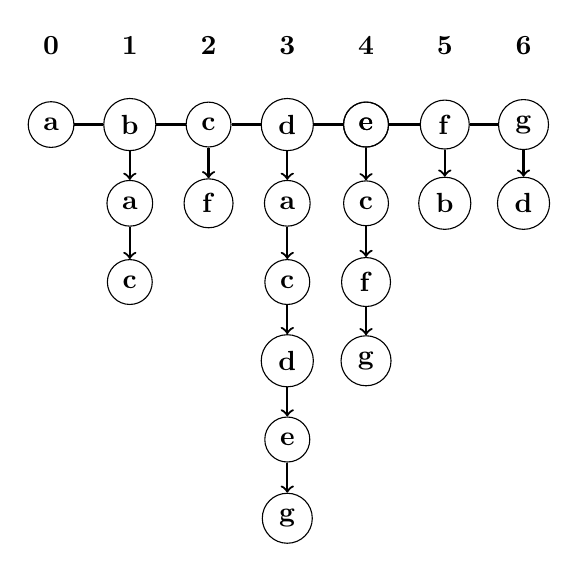
\begin{tikzpicture}
        %a and its adjacents
        \node (k) at (-\scle*3, \scle)     {\textbf{0}};
        \node[shape=circle,draw=black] (a) at (-\scle*3, 0)     {\textbf{a}};
        %b and its adjacents
        \node (l) at (-\scle*2, \scle)     {\textbf{1}};
        \node[shape=circle,draw=black] (b) at (-\scle*2,0)     {\textbf{b}};
        \node[shape=circle,draw=black] (a_1) at (-\scle*2,-\scle)    {\textbf{a}};
        \node[shape=circle,draw=black] (c_2) at (-\scle*2,-\scle*2)  {\textbf{c}};
        %c and its adjacents
        \node (m) at (-\scle, \scle)     {\textbf{2}};
        \node[shape=circle,draw=black] (c) at (-\scle,0)     {\textbf{c}};
        \node[shape=circle,draw=black] (f_1) at (-\scle,-\scle)     {\textbf{f}};
        %d and its adjacents
        \node (n) at (0, \scle)     {\textbf{3}};
        \node[shape=circle,draw=black] (d) at (0,0)     {\textbf{d}};
        \node[shape=circle,draw=black] (a_2) at (0, -\scle)      {\textbf{a}};
        \node[shape=circle,draw=black] (c_3) at (0,-\scle*2)     {\textbf{c}};
        \node[shape=circle,draw=black] (d_2) at (0,-\scle*3)     {\textbf{d}};
        \node[shape=circle,draw=black] (e_1) at (0,-\scle*4)     {\textbf{e}};
        \node[shape=circle,draw=black] (g_2) at (0,-\scle*5)     {\textbf{g}};
        %e and its adjacents
        \node (o) at (\scle,\scle)     {\textbf{4}};
        \node[shape=circle,draw=black] (e) at (\scle,0)     {\textbf{e}};
        \node[shape=circle,draw=black] (e) at (\scle,0)     {\textbf{e}};
        \node[shape=circle,draw=black] (c_1) at (\scle,-\scle)     {\textbf{c}}; 
        \node[shape=circle,draw=black] (f_2) at (\scle,-\scle*2)     {\textbf{f}};
        \node[shape=circle,draw=black] (g_1) at (\scle,-\scle*3)     {\textbf{g}};
        %f and its adjacents
        \node (p) at (\scle*2,\scle)     {\textbf{5}};
        \node[shape=circle,draw=black] (f) at (\scle*2,0)     {\textbf{f}};
        \node[shape=circle,draw=black] (b_1) at (\scle*2,-\scle)     {\textbf{b}};
        %g and its adjacents
        \node (r) at (\scle*3,\scle)     {\textbf{6}};
        \node[shape=circle,draw=black] (g) at (\scle*3,0)     {\textbf{g}};
        \node[shape=circle,draw=black] (d_1) at (\scle*3,-\scle)     {\textbf{d}};
        %connections between
        \path[-, thick] (a) edge (b);
        \path[-, thick] (b) edge (c);
        \path[-, thick] (c) edge (d);
        \path[-, thick] (d) edge (e);
        \path[-, thick] (e) edge (f);
        \path[-, thick] (f) edge (g);
        %adjacents of b
        \path[->, thick] (b) edge (a_1);
        \path[->, thick] (a_1) edge (c_2);
        %adjacents of c
        \path[->, thick] (c) edge (f_1);
        %adjacents of d
        \path[->, thick] (d) edge (a_2);
        \path[->, thick] (a_2) edge (c_3);
        \path[->, thick] (c_3) edge (d_2);
        \path[->, thick] (d_2) edge (e_1);
        \path[->, thick] (e_1) edge (g_2);
        %adjacents of e
        \path[->, thick] (e) edge (c_1);
        \path[->, thick] (c_1) edge (f_2);
        \path[->, thick] (f_2) edge (g_1);
        %adjacents of f
        \path[->, thick] (f) edge (b_1);
        %adjacents of g
        \path[->, thick] (g) edge (d_1);
    \end{tikzpicture}
    	
\end{figure}
\subsection*{b)}
Ordering the vertices $a,b,c,d,e,f,g$
\begin{equation}
    \begin{bmatrix}
        0 & 0 & 0 & 0 & 0 & 0 & 0 \\
        1 & 0 & 1 & 0 & 0 & 0 & 0 \\ 
        0 & 0 & 0 & 0 & 0 & 1 & 0 \\ 
        1 & 0 & 1 & 1 & 1 & 0 & 1 \\ 
        0 & 0 & 1 & 0 & 0 & 1 & 1 \\ 
        0 & 1 & 0 & 0 & 0 & 0 & 0 \\ 
        0 & 0 & 0 & 1 & 0 & 0 & 0 \\ 
    \end{bmatrix}
\end{equation}
\subsection*{c)}
\begin{table}[H]
    \begin{tabular}{|l|l|l|}
        \hline
        \textbf{vertex} & \textbf{indegree} & \textbf{outdegree}\\
        \hline
        $a$ & $2$ & $0$\\
        \hline
        $b$ & $1$ & $2$\\
        \hline
        $c$ & $3$ & $1$\\
        \hline
        $d$ & $2$ & $5$\\
        \hline
        $e$ & $1$ & $3$\\
        \hline
        $f$ & $2$ & $1$\\
        \hline
        $g$ & $2$ & $1$\\
        \hline
    \end{tabular}
\end{table}
\subsection*{d)}
\begin{table}[H]
    \begin{tabular}{l}
        $d-c-f-b-a$\\
        $d-e-f-b-a$\\
        $d-e-g-d-a$\\
        $d-e-g-d-c$\\
        $e-f-b-c-f$\\
        $e-g-d-c-f$\\
    \end{tabular}
\end{table}
\subsection*{e)}
\begin{table}[H]
    \begin{tabular}{l}
        $b-c-f-b$\\
        $c-f-b-c$\\
        $d-d-g-d$\\
        $d-e-c-d$\\
        $d-e-g-d$\\
        $d-g-d-d$\\
        $e-g-d-e$\\
        $f-b-c-f$\\
        $g-d-e-g$\\
        $g-d-d-g$\\
    \end{tabular}
\end{table}
\subsection*{f)}
From the textbook(Eighth Edition) page 717
\\ \\
\begin{tabular}{l}
    \textit{An undirected graph is called connected if there is a path between every pair of distinct}\\
    \textit{vertices of the graph.}   
\end{tabular}
\\ \\
Assume an undirected graph $G=(V,E)$ has two subgraphs $G_1=(V_1,E_1),\ G_2=(V_2,G_2)$ that are weakly connected components of $G$, 
that is there exists an edge $E_1 \in E$ and $E_1=\{v_1,v_2\}$ such that $v_1 \in V_1$ and $v_2 \in V_2$. Further assume, $G_1$ and $G_2$
are both connected graphs. This means every vertex in $G_1$ is reachable from every vertex of $G_1$. This holds also for
$G_2$. Then starting from any vertex of $G_1$, we can reach $v_1$ and for $G_2$, $v_2$. We know $E$ connects $v_1,\ v_2$; then, any 
vertex of $G_1$ is reachable from any vertex of $G_2$ and vice-versa. Hence, $G$ is a connected graph. Therefore, if we prove for 
any undirected graph $G$, its two subgraphs are connected components of $G$, and they are connected subgraphs, we also prove that $G$ is a 
connected graph. From the textbook(Eighth Edition) page 721
\\ \\
\begin{tabular}{l}
    \textit{A directed graph is weakly connected if there is a path between every two vertices in the underlying}\\
    \textit{undirected graph.}   
\end{tabular}
\\ \\
If we prove that there is a path between every two vertices in the underlying undirected graph of the directed graph 
$G$ in the question, in other words that the underlying undirected graph is connected, we also prove that the directed
graph $G$ is weakly connected. We transform the graph into its corresponding undirected graph $H$ and divide it to two 
subgraphs $G_1=(\{a,b,f\},\{\{a,b\},\{b,f\}\})$ and $G_2=(\{c,d,e,g\},\{\{c,d\},\{c,e\},\{d,e\},\{d,g\},\{d,d\},\{e,g\}\})$.
\\ \\
\begin{figure}[H]
    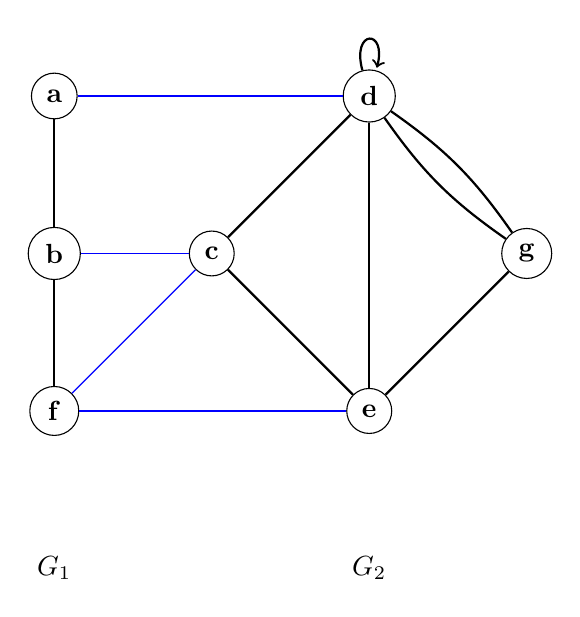
\begin{tikzpicture}
        \node[shape=circle,draw=black] (a) at (-\scale,\scale)     { \textbf{a} };
        \node[shape=circle,draw=black] (b) at (-\scale,0)     {\textbf{b}};
        \node[shape=circle,draw=black] (c) at (0, 0)     {\textbf{c}};
        \node[shape=circle,draw=black] (d) at (\scale,\scale)     {\textbf{d}};
        \node[shape=circle,draw=black] (e) at (\scale, -\scale)     {\textbf{e}};
        \node[shape=circle,draw=black] (f) at (-\scale,-\scale)     {\textbf{f}};
        \node[shape=circle,draw=black] (g) at (\scale*2,0)     {\textbf{g}};
        %labels
        \node (k) at (-\scale,-\scale*2)     {\textbf{$G_1$}};
        \node (l) at (\scale,-\scale*2)     {\textbf{$G_2$}};
        %edges within the subgraphs
        \path[-, thick] (a) edge (b);
        \path[-, thick] (b) edge (f);
        
        \path[-, thick] (c) edge (d);
        \path[-, thick] (d) edge (e);
        \path[-, thick] (d) edge [loop above](d);
        \path[-, thick] (e) edge (c);
        \path[-, thick] (g) edge [bend left=10](d);
        \path[-, thick] (g) edge [bend right=10](d);
        \path[-, thick] (g) edge (e);
        %edges between the subgraphs
        \path[-,draw=blue] (a) edge (d);
        \path[-,draw=blue] (b) edge (c);
        \path[-,draw=blue] (f) edge (c);
        \path[-,draw=blue] (f) edge (e);
	\end{tikzpicture}
\end{figure}
Similarly, we divide $G_2$ into subgraphs $G_3=(\{c,d\},\{\{c,d\},\{d,d\}\})$ and $G_4=(\{e,g\},\{\{e,g\}\})$.
We can traverse between $c$ and $d$ through the edge $\{c,d\}$, then $G_3$ is connected. Similarly, 
we can traverse between $e$ and $g$ through the edge $\{e,g\}$, then $G_4$ is connected. $G_3$ and
$G_4$ are connected via the edges $\{c,e\},\{d,e\}$ and $\{d,g\}$ with multiplicity of $2$; hence, $G_2$ is connected. 
Vertices $a$ and $b$ are adjacent, we can traverse from $a$ to $b$, Vertices $b$ and $f$ are adjacent, we can traverse 
from $b$ to $f$, then we can traverse from $a$ to $f$ also; hence $G_1$ is connected. $G_1$ and
$G_2$ are connected via the edges $\{a,d\},\{b,c\},\{c,f\},\{e,f\}$; hence, $H$ is connected. We conclude that
the underlying undirected graph $H$ of the directed graph $G$ is connected, hence the directed graph $G$ is weakly connected.
\subsection*{g)}
\begin{figure}[H]
    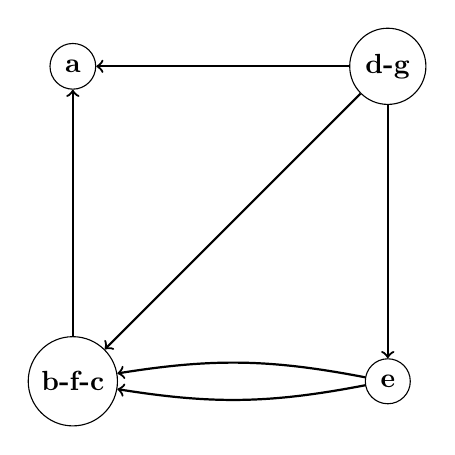
\begin{tikzpicture}
        \node[shape=circle,draw=black] (a) at (-\scale,\scale)     { \textbf{a} };
        \node[shape=circle,draw=black] (b) at (-\scale,-\scale)     {\textbf{b-f-c}};
        \node[shape=circle,draw=black] (d) at (\scale,\scale)     {\textbf{d-g}};
        \node[shape=circle,draw=black] (e) at (\scale, -\scale)     {\textbf{e}};

        %edges within the subgraphs
        \path[->, thick] (b) edge (a);
        \path[->, thick] (d) edge (a);
        \path[->, thick] (d) edge (b);
        \path[->, thick] (d) edge (e);
        \path[->, thick] (e) edge [bend left=10](b);
        \path[->, thick] (e) edge [bend right=10](b);
	\end{tikzpicture}
\end{figure}
\subsection*{h)}

\section*{Answer 3}
\subsection*{a)}
From the textbook(Eighth Edition) page 729
\\ \\
\begin{tabular}{l}
    \textit{An Euler path in G is a simple path containing every edge of G.}   
\end{tabular}
\\ \\
The simple path $d-c-b-d-e-f-g-h-e-d-a-b$ is an Euler path, since it contains every edge of $G$.
Then $G$ has an Euler Path.
\subsection*{b)}
From the textbook(Eighth Edition) page 729
\\ \\
\begin{tabular}{l}
    \textit{A connected multigraph with at least two vertices has an Euler circuit if and only if each of} \\
    \textit{its vertices has even degree.}   
\end{tabular}
\\ \\
$G$ has $8$ vertices, more than two. Since the vertex $b$ has $3$ edges incident with it, then its degree is
$3$, which is odd. Then $G$ does not have any Euler circuits 
\subsection*{c)}
From the textbook(Eighth Edition) page 734
\\ \\
\begin{tabular}{l}
    \textit{A simple path in a graph G that passes through every vertex exactly once is called a Hamilton}\\
    \textit{path.} 
\end{tabular}
\\ \\
The simple path $a-b-c-d-e-f-g-h$ is a Hamiltonian path, since it passes through every vertex of $G$ once.
Then $G$ has an Hamiltonian Path.
\subsection*{d)}
From the textbook(Eighth Edition) page 734
\\ \\
\begin{tabular}{l}
    \textit{A simple circuit in a graph G that passes through every vertex exactly once is called a Hamilton circuit.}  
\end{tabular}
\\ \\
Let us observe two subgraphs of $G$, namely $G_1=\{V_1,E_1\}=\{\{a,b,c,d\},\{\{a,b\},\{b,c\},\{c,d\},\{b,d\},\{a,d\}\}\}$, 
$G_2=\{V_2,E_2\}=\{\{e,f,g,h\},\{\{e,f\},\{f,g\},\{g,h\},\{e,h\}\}\}$. Assume $G$ has a 
Hamiltonian circuit with an initial vertex $v_0$. 
\\ \\
\begin{tabular}{l}
    The circuit should pass through $d$ and $e$ exactly once (*).\\
    The circuit should pass through every vertex of $G_1$ and $G_2$ exactly once (**).
\end{tabular}
\\ \\
If $v_0 \in G_1$, since circuit passes through $d$ and $e$ exactly once, it must terminate at a vertex of $G_2$, in order
to pass through every vertex of $G_2$; however, $v_0 \notin V_2$, then this path is not a circuit. 
\\ \\
Similarly if $v_0 \in G_2$, since circuit passes through $d$ and $e$ exactly once, it must terminate at a 
vertex of $G_1$; however, $v_0 \notin V_1$. Then, by using (*) and (**), we disprove
that there is such a circuit. Then, there exists no such circuit. 
Hence by contradiction, $G$ has no Hamilton circuits.

\section*{Answer 4}
From a work of David Glickenstein, namely "Graph Theory Notes 5: Graphs as matrices, 
spectral graph theory, and PageRank", at page 1 \label{work}
\\ \\
\begin{tabular}{l}
    \textbf{Definition 1 }\textit{A permutation matrix is a matrix gotten from the identity by permuting the columns } \\
    \textit{(i.e., switching some of the columns).}   
\end{tabular}
\\ \\
\begin{tabular}{l}
    \textbf{Proposition 2 }\textit{The graphs $G$ and $G'$ are isomorphic if and only if their adjacency} \\
    \textit{matrices are related by} \\
    \\
    $\quad A=P^TA'P \quad (*)$\\
    \\
    \textit{for some permutation matrix $P$.}
\end{tabular}
\\ \\
In our case, adjacency matrix of $G$, Ordering the vertices $a,b,c,d,e$
\begin{equation}
    \begin{bmatrix}
        0 & 1 & 0 & 0 & 1 \\
        1 & 0 & 1 & 0 & 0 \\
        0 & 1 & 0 & 1 & 0 \\
        0 & 0 & 1 & 0 & 1 \\
        1 & 0 & 0 & 1 & 0 \\ 
    \end{bmatrix}
\end{equation}
adjacency matrix of $G'$, Ordering the vertices $a',b',c',d',e'$
\begin{equation}
    \begin{bmatrix}
        0 & 1 & 0 & 0 & 1 \\
        1 & 0 & 1 & 0 & 0 \\
        0 & 1 & 0 & 1 & 0 \\
        0 & 0 & 1 & 0 & 1 \\
        1 & 0 & 0 & 1 & 0 \\ 
    \end{bmatrix}
\end{equation}
We observe that $G=G'$. Then the permutation matrix $P$ can be $5$x$5$ identity matrix, 
holding the equality (*). Since there exists such permutation matrix $P=I$, $G$ an $G'$
are isomorphic. 
\\ \\
Work of David Glickenstein can be accessed via the below link
\\ \\
\begin{tabular}{l}
    https://www.math.arizona.edu/(tilde)glickenstein/math443f14/notes5matrices.pdf
\end{tabular}
\\ \\
\textbf{NOTE:} Please change (tilde) with tilde sign -ascii of the character is 126- in order to access. 
I could not have the full url link with tilde sign, since I was not allowed to use extra packages such as
the url package.
\section*{Answer 5}
\subsection*{a)}
A pseudocode for Djikstra's Algorithm is below and at each step, variables are shown with a table below 
that contains the values of the vertices and previous vertices that are connected to them
in the shortest path from the initial vertex. The tables below show the values after the operations 
done at each step. (*) sign before the vertices' labels, mark adjacent unvisited vertices, since at each 
step only possible elements that are subject to change are adjacent unvisited vertices.
\\ \\
\textbf{Pseudocode for Djikstra's Algorithm}
\\ \\
At initial step, assign $0$ for the initial vertex, $\infty$ for other vertices.
\\ \\
At each step do the following(s)
\\ \\
\textbf{1)}Take the vertex which has the minimum value in unvisited vertices, as the next vertex
-Assuming that the vertices are sorted, then in case of equality, first one is chosen.\\
\textbf{2)}if the next vertex is None (the set of unvisited vertices is empty), halt\\
\textbf{3)}else if the current vertex is None, assign next vertex to current vertex, pop current vertex
from unvisited vertices pushing it to visited vertices and continue (proceed to the next step) \\
\textbf{4)}else proceed for each vertex in unvisited adjacent vertices, assign next vertex to current vertex
, pop current vertex from unvisited vertices pushing it to visited vertices and continue
\\ \\
\textbf{Initial step (0)} Current vertex: None\\
Next vertex: a\\
Visited vertices: \{\}\\
Unvisited vertices: \{a,b,c,d,e,f,g,h,i,j,k\}\\
Adjacent vertices that are unvisited: \{\}\\
\begin{tabular}{|l|l|l|}
    \hline
    vertex & distance & previous \\
    \hline
    a & $0$ &  \\
    \hline
    b & $\infty$ &  \\
    \hline
    c & $\infty$ &  \\
    \hline
    d & $\infty$ &  \\
    \hline
    e & $\infty$ &  \\
    \hline
    f & $\infty$ &  \\
    \hline
    g & $\infty$ &  \\
    \hline
    h & $\infty$ &  \\
    \hline
    i & $\infty$ &  \\
    \hline
    j & $\infty$ &  \\
    \hline
    k & $\infty$ &  \\
    \hline
\end{tabular}
\\ \\
\\ \\
\textbf{Step (1)} Current vertex: a\\
Next vertex: b\\
Visited vertices: \{a\}\\
Unvisited vertices: \{b,c,d,e,f,g,h,i,j,k\}\\
Adjacent vertices that are unvisited: \{b,e,h\}\\
\begin{tabular}{|l|l|l|}
    \hline
    vertex & distance & previous \\
    \hline
    a & $0$ &  \\
    \hline
    *b & $3$ & a \\
    \hline
    c & $\infty$ &  \\
    \hline
    d & $\infty$ &  \\
    \hline
    *e & $5$ & a \\
    \hline
    f & $\infty$ &  \\
    \hline
    g & $\infty$ &  \\
    \hline
    *h & $8$ & a \\
    \hline
    i & $\infty$ &  \\
    \hline
    j & $\infty$ &  \\
    \hline
    k & $\infty$ &  \\
    \hline
\end{tabular}
\\ \\
\\ \\
\textbf{Step (2)} Current vertex: b\\
Next vertex: c\\
Visited vertices: \{a,b\}\\
Unvisited vertices: \{c,d,e,f,g,h,i,j,k\}\\
Adjacent vertices that are unvisited: \{c,e,f\}\\
\begin{tabular}{|l|l|l|}
    \hline
    vertex & distance & previous \\
    \hline
    a & $0$ &  \\
    \hline
    b & $3$ & a \\
    \hline
    *c & $5$ & b \\
    \hline
    d & $\infty$ &  \\
    \hline
    *e & $5$ & a \\
    \hline
    *f & $10$ & b \\
    \hline
    g & $\infty$ &  \\
    \hline
    h & $8$ & a \\
    \hline
    i & $\infty$ &  \\
    \hline
    j & $\infty$ &  \\
    \hline
    k & $\infty$ &  \\
    \hline
\end{tabular}
\\ \\
\\ \\
\textbf{Step (3)} Current vertex: c\\
Next vertex: e\\
Visited vertices: \{a,b,c\}\\
Unvisited vertices: \{d,e,f,g,h,i,j,k\}\\
Adjacent vertices that are unvisited: \{d,f,g\}\\
\begin{tabular}{|l|l|l|}
    \hline
    vertex & distance & previous \\
    \hline
    a & $0$ &  \\
    \hline
    b & $3$ & a \\
    \hline
    c & $5$ & b \\
    \hline
    *d & $8$ & c \\
    \hline
    e & $5$ & a \\
    \hline
    *f & $7$ & c \\
    \hline
    *g & $11$ & c \\
    \hline
    h & $8$ & a \\
    \hline
    i & $\infty$ &  \\
    \hline
    j & $\infty$ &  \\
    \hline
    k & $\infty$ &  \\
    \hline
\end{tabular}
\\ \\
\\ \\
\textbf{Step (4)} Current vertex: e\\
Next vertex: f\\
Visited vertices: \{a,b,c,e\}\\
Unvisited vertices: \{d,f,g,h,i,j,k\}\\
Adjacent vertices that are unvisited: \{f,h\}\\
\begin{tabular}{|l|l|l|}
    \hline
    vertex & distance & previous \\
    \hline
    a & $0$ &  \\
    \hline
    b & $3$ & a \\
    \hline
    c & $5$ & b \\
    \hline
    d & $8$ & c \\
    \hline
    e & $5$ & a \\
    \hline
    *f & $7$ & c \\
    \hline
    g & $11$ & c \\
    \hline
    *h & $8$ & a \\
    \hline
    i & $\infty$ &  \\
    \hline
    j & $\infty$ &  \\
    \hline
    k & $\infty$ &  \\
    \hline
\end{tabular}
\\ \\
\\ \\
\textbf{Step (5)} Current vertex: f\\
Next vertex: d\\
Visited vertices: \{a,b,c,e,f\}\\
Unvisited vertices: \{d,g,h,i,j,k\}\\
Adjacent vertices that are unvisited: \{g,h,i,j\}\\
\begin{tabular}{|l|l|l|}
    \hline
    vertex & distance & previous \\
    \hline
    a & $0$ &  \\
    \hline
    b & $3$ & a \\
    \hline
    c & $5$ & b \\
    \hline
    d & $8$ & c \\
    \hline
    e & $5$ & a \\
    \hline
    f & $7$ & c \\
    \hline
    *g & $11$ & c \\
    \hline
    *h & $8$ & a \\
    \hline
    *i & $11$ & f \\
    \hline
    *j & $10$ & f \\
    \hline
    k & $\infty$ &  \\
    \hline
\end{tabular}
\\ \\
\\ \\
\textbf{Step (6)} Current vertex: d\\
Next vertex: h\\
Visited vertices: \{a,b,c,e,f,d\}\\
Unvisited vertices: \{g,h,i,j,k\}\\
Adjacent vertices that are unvisited: \{g,k\}\\
\begin{tabular}{|l|l|l|}
    \hline
    vertex & distance & previous \\
    \hline
    a & $0$ &  \\
    \hline
    b & $3$ & a \\
    \hline
    c & $5$ & b \\
    \hline
    d & $8$ & c \\
    \hline
    e & $5$ & a \\
    \hline
    f & $7$ & c \\
    \hline
    *g & $11$ & c \\
    \hline
    h & $8$ & a \\
    \hline
    i & $11$ & f \\
    \hline
    j & $10$ & f \\
    \hline
    *k & $10$ & d \\
    \hline
\end{tabular}
\\ \\
\\ \\
\textbf{Step (7)} Current vertex: h\\
Next vertex: i\\
Visited vertices: \{a,b,c,e,f,d,h\}\\
Unvisited vertices: \{g,i,j,k\}\\
Adjacent vertices that are unvisited: \{i\}\\
\begin{tabular}{|l|l|l|}
    \hline
    vertex & distance & previous \\
    \hline
    a & $0$ &  \\
    \hline
    b & $3$ & a \\
    \hline
    c & $5$ & b \\
    \hline
    d & $8$ & c \\
    \hline
    e & $5$ & a \\
    \hline
    f & $7$ & c \\
    \hline
    g & $11$ & c \\
    \hline
    h & $8$ & a \\
    \hline
    *i & $10$ & h \\
    \hline
    j & $10$ & f \\
    \hline
    k & $10$ & d \\
    \hline
\end{tabular}
\\ \\
\\ \\
\textbf{Step (8)} Current vertex: i\\
Next vertex: j\\
Visited vertices: \{a,b,c,e,f,d,h,i\}\\
Unvisited vertices: \{g,j,k\}\\
Adjacent vertices that are unvisited: \{j\}\\
\begin{tabular}{|l|l|l|}
    \hline
    vertex & distance & previous \\
    \hline
    a & $0$ &  \\
    \hline
    b & $3$ & a \\
    \hline
    c & $5$ & b \\
    \hline
    d & $8$ & c \\
    \hline
    e & $5$ & a \\
    \hline
    f & $7$ & c \\
    \hline
    g & $11$ & c \\
    \hline
    h & $8$ & a \\
    \hline
    i & $10$ & h \\
    \hline
    *j & $10$ & f \\
    \hline
    k & $10$ & d \\
    \hline
\end{tabular}
\\ \\
\\ \\
\textbf{Step (9)} Current vertex: j\\
Next vertex: k\\
Visited vertices: \{a,b,c,e,f,d,h,i,j\}\\
Unvisited vertices: \{g,k\}\\
Adjacent vertices that are unvisited: \{g,k\}\\
\begin{tabular}{|l|l|l|}
    \hline
    vertex & distance & previous \\
    \hline
    a & $0$ &  \\
    \hline
    b & $3$ & a \\
    \hline
    c & $5$ & b \\
    \hline
    d & $8$ & c \\
    \hline
    e & $5$ & a \\
    \hline
    f & $7$ & c \\
    \hline
    *g & $11$ & c \\
    \hline
    h & $8$ & a \\
    \hline
    i & $10$ & h \\
    \hline
    j & $10$ & f \\
    \hline
    *k & $10$ & d \\
    \hline
\end{tabular}
\\ \\
\\ \\
\textbf{Step (10)} Current vertex: k\\
Next vertex: g\\
Visited vertices: \{a,b,c,e,f,d,h,i,j,k\}\\
Unvisited vertices: \{g\}\\
Adjacent vertices that are unvisited: \{g\}\\
\begin{tabular}{|l|l|l|}
    \hline
    vertex & distance & previous \\
    \hline
    a & $0$ &  \\
    \hline
    b & $3$ & a \\
    \hline
    c & $5$ & b \\
    \hline
    d & $8$ & c \\
    \hline
    e & $5$ & a \\
    \hline
    f & $7$ & c \\
    \hline
    *g & $11$ & c \\
    \hline
    h & $8$ & a \\
    \hline
    i & $10$ & h \\
    \hline
    j & $10$ & f \\
    \hline
    k & $10$ & d \\
    \hline
\end{tabular}
\\ \\
\\ \\
\textbf{Step (11)} Current vertex: g\\
Next vertex: None\\
Visited vertices: \{a,b,c,e,f,d,h,i,j,k,g\}\\
Unvisited vertices: \{\}\\
Adjacent vertices that are unvisited: \{\}\\
\begin{tabular}{|l|l|l|}
    \hline
    vertex & distance & previous \\
    \hline
    a & $0$ &  \\
    \hline
    b & $3$ & a \\
    \hline
    c & $5$ & b \\
    \hline
    d & $8$ & c \\
    \hline
    e & $5$ & a \\
    \hline
    f & $7$ & c \\
    \hline
    *g & $11$ & c \\
    \hline
    h & $8$ & a \\
    \hline
    i & $10$ & h \\
    \hline
    j & $10$ & f \\
    \hline
    k & $10$ & d \\
    \hline
\end{tabular}
\\ \\
After halting, we observe the last state of the variables in the above table. Starting from 
the terminal vertex, if the values are to be backtracked by checking their previous vertices 
on the table (i.e., j to f, f to c and so forth), then we see the path
\\ \\
\begin{tabular}{l}
    $a-b-c-f-j$
\end{tabular}
\\ \\
is to shortest path, from $a$ to $j$.
\subsection*{b)}

The procedure for Prim's algorithm is as below
\\ \\
At initial step, remove a random initial vertex from unvisited vertices -preferably the first 
element in the list, and push it to visited vertices.
\\ \\
At each step do the following(s)
\\ \\
\textbf{1)}Halt if unvisited vertices is empty\\
\textbf{2)}Inspect every edge that connects a visited vertex to an unvisited vertex \\
\textbf{3)}Pick the edge with the least weight and store it in the visited edges 
-Assuming that the vertices are sorted, then in case of equality, first one is chosen\\
\textbf{4)}Pop the unvisited vertex that the chosen edge is incident to and push it to 
visited vertices.\\
\textbf{5)}Proceed to the next step\\
\\ \\
\textbf{Initial step (0)} 
Visited vertices: \{\}\\
Visited edges: \{\}\\
Unvisited vertices: \{a,b,c,d,e,f,g,h,i,j,k\}\\
Adjacent vertices that are unvisited: \{\}\\
\\ \\
\textbf{Step (1)} 
Visited vertices: \{a\}\\
Visited edges: \{\}\\
Unvisited vertices: \{b,c,d,e,f,g,h,i,j,k\}\\
Adjacent vertices that are unvisited: \{\{a,b\},\{a,e\},\{a,h\}\}\\
\{a,b\} has the minimum weight.
\\ \\
\textbf{Step (2)} 
Visited vertices: \{a,b\}\\
Visited edges: \{\{a,b\}\}\\
Unvisited vertices: \{c,d,e,f,g,h,i,j,k\}\\
Adjacent vertices that are unvisited: \{\{a,e\},\{a,h\},\{b,c\},\{b,e\},\{b,f\}\}\\
\{b,c\} has the minimum weight.
\\ \\
\textbf{Step (3)} 
Visited vertices: \{a,b,c\}\\
Visited edges: \{\{a,b\},\{b,c\}\}\\
Unvisited vertices: \{d,e,f,g,h,i,j,k\}\\
Adjacent vertices that are unvisited: \{\{a,e\},\{a,h\},\{b,e\},\{b,f\},\{c,d\},\{c,f\},\{c,g\}\}\\
\{c,f\} has the minimum weight.
\\ \\
\textbf{Step (4)} 
Visited vertices: \{a,b,c,f\}\\
Visited edges: \{\{a,b\},\{b,c\},\{c,f\}\}\\
Unvisited vertices: \{d,e,g,h,i,j,k\}\\
Adjacent vertices that are unvisited: \{\{a,e\},\{a,h\},\{b,e\},\{c,d\},\{c,g\}\}\\
\{c,d\} has the minimum weight.
\\ \\
\textbf{Step (5)} 
Visited vertices: \{a,b,c,d,f\}\\
Visited edges: \{\{a,b\},\{b,c\},\{c,f\},\{c,d\}\}\\
Unvisited vertices: \{e,g,h,i,j,k\}\\
Adjacent vertices that are unvisited: \{\{a,e\},\{a,h\},\{b,e\},\{c,g\}\,\{d,g\},\{d,k\},\{f,e\},\{f,g\},\{f,h\},\{f,i\},\{f,j\}\}\\
\{d,k\} has the minimum weight.
\\ \\
\textbf{Step (6)} 
Visited vertices: \{a,b,c,d,f,k\}\\
Visited edges: \{\{a,b\},\{b,c\},\{c,f\},\{c,d\},\{d,k\}\}\\
Unvisited vertices: \{e,g,h,i,j\}\\
Adjacent vertices that are unvisited: \{\{a,e\},\{a,h\},\{b,e\},\{c,g\}\,\{d,g\},\{f,e\},\{f,g\},\{f,h\},\{f,i\},\{f,j\},\{k,g\},\{k,j\}\}\\
\{f,j\} has the minimum weight.
\\ \\
\textbf{Step (7)} 
Visited vertices: \{a,b,c,d,f,j,k\}\\
Visited edges: \{\{a,b\},\{b,c\},\{c,f\},\{c,d\},\{d,k\},\{f,j\}\}\\
Unvisited vertices: \{e,g,h,i\}\\
Adjacent vertices that are unvisited: \{\{a,e\},\{a,h\},\{b,e\},\{c,g\}\,\{d,g\},\{f,e\},\{f,g\},\{f,h\},\{f,i\},\{k,g\},\{j,g\},\{j,i\}\}\\
\{f,e\} has the minimum weight.
\\ \\
\textbf{Step (8)} 
Visited vertices: \{a,b,c,d,e,f,j,k\}\\
Visited edges: \{\{a,b\},\{b,c\},\{c,f\},\{c,d\},\{d,k\},\{f,j\},\{f,e\}\}\\
Unvisited vertices: \{g,h,i\}\\
Adjacent vertices that are unvisited: \{\{a,h\},\{d,g\},\{e,h\},\{f,g\},\{f,h\},\{f,i\},\{j,g\},\{j,i\}\}\\
\{f,g\} has the minimum weight.
\\ \\
\textbf{Step (9)} 
Visited vertices: \{a,b,c,d,e,f,g,j,k\}\\
Visited edges: \{\{a,b\},\{b,c\},\{c,f\},\{c,d\},\{d,k\},\{f,g\},\{f,j\},\{f,e\}\}\\
Unvisited vertices: \{h,i\}\\
Adjacent vertices that are unvisited: \{\{a,h\},\{e,h\},\{f,h\},\{f,i\},\{j,i\}\}\\
\{f,i\} has the minimum weight.
\\ \\
\textbf{Step (10)} 
Visited vertices: \{a,b,c,d,e,f,g,i,j,k\}\\
Visited edges: \{\{a,b\},\{b,c\},\{c,f\},\{c,d\},\{d,k\},\{f,g\},\{f,j\},\{f,e\},\{f,i\}\}\\
Unvisited vertices: \{h\}\\
Adjacent vertices that are unvisited: \{\{a,h\},\{e,h\},\{f,h\}\},\{i,h\}\}\\
\{i,h\} has the minimum weight.
\\ \\
\textbf{Step (11)} 
Visited vertices: \{a,b,c,d,e,f,g,h,i,j,k\}\\
Visited edges: \{\{a,b\},\{b,c\},\{c,f\},\{c,d\},\{d,k\},\{f,g\},\{f,j\},\{f,e\},\{f,i\},\{f,h\}\}\\
Unvisited vertices: \{\}\\
Adjacent vertices that are unvisited: \{\}\\
\\ \\
After halting, connecting the visited edges by their common vertices, we have a minimum spanning
tree for the initial vertex A.
\\ \\
\begin{figure}[H]
    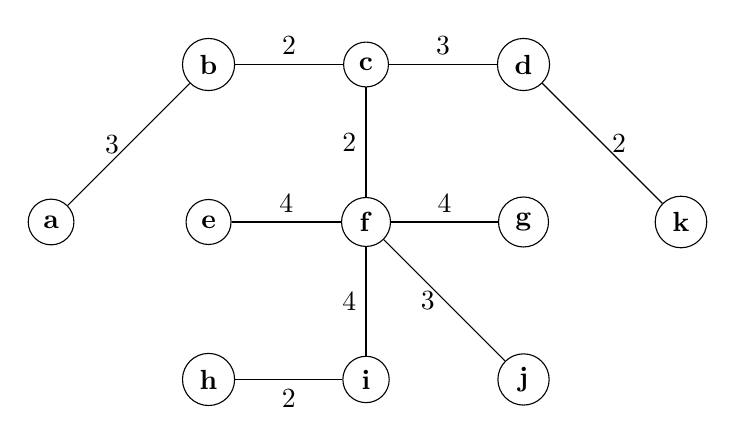
\begin{tikzpicture}
        \node[shape=circle,draw=black] (a) at (-\scale*2,0)     { \textbf{a} };
        \node[shape=circle,draw=black] (b) at (-\scale,\scale)     {\textbf{b}};
        \node[shape=circle,draw=black] (c) at (0,\scale)     {\textbf{c}};
        \node[shape=circle,draw=black] (d) at (\scale,\scale)     {\textbf{d}};
        \node[shape=circle,draw=black] (e) at (-\scale,0)     {\textbf{e}};
        \node[shape=circle,draw=black] (f) at (0,0)     {\textbf{f}};
        \node[shape=circle,draw=black] (g) at (\scale,0)     {\textbf{g}};
        \node[shape=circle,draw=black] (h) at (-\scale,-\scale)     { \textbf{h} };
        \node[shape=circle,draw=black] (i) at (0,-\scale)     {\textbf{i}};
        \node[shape=circle,draw=black] (j) at (\scale,-\scale)     {\textbf{j}};
        \node[shape=circle,draw=black] (k) at (\scale*2,0)     {\textbf{k}};

        %edges with text
        \path[-] (a) edge node[left]{3} (b);
	    \path[-] (b) edge node[above]{2} (c);
	    \path[-] (e) edge node[above]{4} (f);	
	    \path[-] (h) edge node[below]{2} (i);	
	    \path[-] (c) edge node[above]{3} (d);
	    \path[-] (c) edge node[left]{2} (f);
	    \path[-] (f) edge node[above]{4} (g);
	    \path[-] (f) edge node[left]{3} (j);
	    \path[-] (f) edge node[left]{4} (i);	
	    \path[-] (d) edge node[right]{2} (k);
	\end{tikzpicture}
\end{figure}
\section*{Answer 6}
\subsection*{a)}
There are $7$ vertices, and $6$ edges in $T$. $f$ and $g$ have largest levels, $3$; then
height of $T$ is $3$. 
\subsection*{b)}
a-b-c-d-e-f-g
\subsection*{c)}
b-d-f-g-e-c-a
\subsection*{d)}
b-a-d-c-f-e-g
\subsection*{e)}
From the textbook(Eighth Edition) page 783-784
\\ \\
\begin{tabular}{l}
    \textit{In a rooted tree, Vertices that have children are called internal vertices.} (1)\\
    \textit{The tree is called a full m-ary tree if every internal vertex has exactly m children. An m-ary} (2)\\
    \textit{tree with $m = 2$ is called a binary tree.} (3)     
\end{tabular}
\\ \\
In question, a is given as a root, then the tree is a rooted tree. 
Using (1), we see that a, c, e are internal vertices. Vertices a, c and e have two children ($m=2$), then 
the given tree is a full binary tree.
\subsection*{f)}
From the textbook(Eighth Edition) page 792, question $27$
\\ \\
\begin{tabular}{l}
    \textit{A complete m-ary tree is a full m-ary tree in which every leaf is at the same level.} (1)\\
\end{tabular}
\\ \\
From the textbook(Eighth Edition) page 783
\\ \\
\begin{tabular}{l}
    \textit{A vertex of a rooted tree is called a leaf if it has no children.} (2)\\
\end{tabular}
\\ \\
Leaves of the given tree are b, d, f, g. b, d and f are at different levels; hence, $T$ is not a
complete tree, then not a complete binary tree.
\subsection*{g)}

From the textbook(Eighth Edition) page 794, binary search trees have the following property
\\ \\
\begin{tabular}{l}
    \textit{Vertices are assigned keys so that the key of a vertex is both larger than the keys of all vertices}\\
    \textit{in its left subtree and smaller than the keys of all vertices in its right subtree.}
\end{tabular}
\\ \\
\textbf{NOTE} Below, the term \textit{ordered} or \textit{sorted} is used for a sequence, when 
for every two values $a$ and $b$ in the sequence, if $a$ is on the left of $b$, then $a \leq b$.
\\ \\
\textbf{Lemma 1} An in-order traversal of a binary search tree with vertices that have unique keys
always prints the vertices of the tree in sorted order
\\ \\
\textbf{Proof by induction}\\ 
\textbf{BASE STEP} Printing a single vertex gives a sorted list with a length $1$\\
\textbf{INDUCTIVE STEP} Assume An in-order traversal of a binary search tree with 
$1,2,3...k$ vertices that have unique keys always prints the vertices of the tree in sorted order. 
Assume an additional vertex $a$ with a unique key is inserted. If we print the subtree $T_a$ that
$a$ is the root of, in inorder, we print $a$ in the middle, subtree with smaller values than 
$a$ on the left, subtree with larger values on the right. We know that inorder print of both 
subtrees of $a$ are ordered, since their number of vertices $n$ is less than or equal to $k$
- assuming an empty list is also ordered (trivial case $n=0$). Then 
inorder print of $T_a$ is ordered. Similarly we print the parent of $a$ in the middle, 
$T_a$ to the left if each value of $T_a$ is smaller than of parent of $a$, right if larger, 
in inorder traversal. 
Then inorder print of $T_p$, the tree that parent of $a$ is root of, is also ordered. 
We know that inorder print of remaining vertices of the tree 
was already ordered, before the insertion. Then inorder print of the new tree is also ordered, 
completing the proof.
\\ \\
Let us observe the sequence b,a,d,c,f,e,g which is obtained by inorder traversal in part \textbf{(d)}.
Substituting their values,the sequence becomes $13,17,19,24,23,43,58$ -every key is unique. The sequence is not ordered, since
$24$ is on the left of $23$, but $24 \leq 23$ does not hold. Then, by \textit{Lemma 1}, $T$ is not a binary search tree.
\subsection*{h)}
the minimum number of nodes for a full binary tree with height $5$ is $2*height+1=2*5+1=11$
\subsection*{i)}
\begin{figure}[H]
    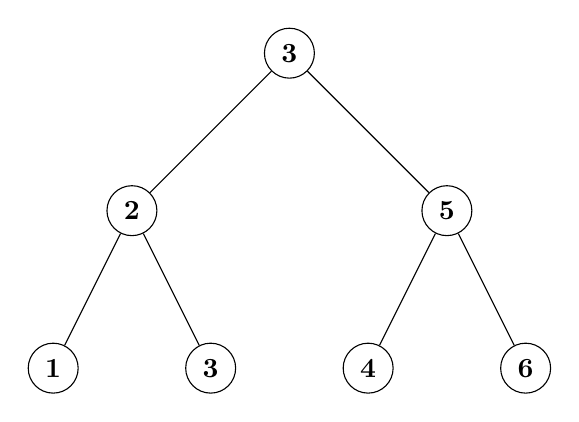
\begin{tikzpicture}
        \node[shape=circle,draw=black] (a) at (-\scle*3,0)     { \textbf{1} };
        \node[shape=circle,draw=black] (b) at (-\scle*2,\scle*2)     {\textbf{2}};
        \node[shape=circle,draw=black] (c) at (-\scle,0)     {\textbf{3}};
        \node[shape=circle,draw=black] (d) at (0,\scle*4)     {\textbf{3}};
        \node[shape=circle,draw=black] (e) at (\scle,0)     {\textbf{4}};
        \node[shape=circle,draw=black] (f) at (\scle*2,\scle*2)     {\textbf{5}};
        \node[shape=circle,draw=black] (g) at (\scle*3,0)     {\textbf{6}};
        

        %edges with text
        \path[-] (a) edge (b);
	    \path[-] (b) edge (c);
	    \path[-] (b) edge (d);	
	    \path[-] (d) edge (f);	
	    \path[-] (f) edge (e);
	    \path[-] (f) edge (g);
	   
	\end{tikzpicture}
\end{figure}
\subsection*{j)}
The last value is the value found, and values before are the values compared with the key.
To find key $1$, $3,2,1$
To find key $6$, $3,5,6$
\subsection*{k)}

\begin{figure}[H]
	\centering
	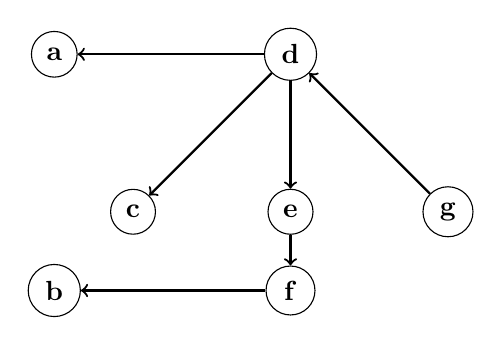
\begin{tikzpicture}
	
	\node[shape=circle,draw=black] (a) at (0, 3)     {\textbf{a}};
	\node[shape=circle,draw=black] (b) at (0, 0)     {\textbf{b}};
	\node[shape=circle,draw=black] (c) at (1, 1)     {\textbf{c}};
	\node[shape=circle,draw=black] (d) at (3, 3)     {\textbf{d}};
	\node[shape=circle,draw=black] (e) at (3, 1)     {\textbf{e}};
	\node[shape=circle,draw=black] (f) at (3, 0)     {\textbf{f}};
	\node[shape=circle,draw=black] (g) at (5, 1)     {\textbf{g}};

	\path[->, thick] (g) edge (d);
	\path[->, thick] (d) edge (a);
	\path[->, thick] (d) edge (c);
	\path[->, thick] (d) edge (e);
	\path[->, thick] (e) edge (f);
	\path[->, thick] (f) edge (b);
	
	\end{tikzpicture} 
\end{figure}
$g$ is the root
\subsection*{l)}
From the textbook(Eighth Edition) page 789
\\ \\
\begin{tabular}{l}
    \textit{The height of a rooted tree is the maximum of the levels of vertices. In other words, the height of} \\  
    \textit{a rooted tree is the length of the longest path from the root to any vertex.}  
\end{tabular}
\\ \\
The longest possible length from the root of a rooted tree with $k$ vertices is $k-1$.
\\ \\
\textbf{Proof by induction}\\
\textbf{BASE STEP} A single vertex is a tree, has $1-1=0$ height, which is the maximum possible height.\\
\textbf{INDUCTIVE STEP} Assume the longest possible length from the root of a rooted tree with $t$ vertices is $t-1$.
If, an additional vertex is inserted as a child of the most distant vertex (from the root), the height $h = t$, 
else $h = t-1$. Then, the longest possible length from the root of a rooted tree with 
$t+1$ vertices is $t$, completing the proof.   
\end{document}

​

